% Chapter 2_0

\chapter{Fundamentação Teórica} % Main chapter title
\label{chap:Chapter2_0} % For referencing the chapter elsewhere, use \ref{chap:Chapter2_0} 

	\todo[inline]{Remover este capitulo e passar info para estado da arte..}

	Este capítulo apresenta os principais conceitos teóricos necessários para compreender o trabalho desenvolvido. Começa-se por uma breve introdução aos \textit{Large Language Models (LLMs)}, incluindo as suas principais limitações e as arquiteturas disponiveis para os adaptar, como o Prompt Engineering, o \gls{RAG} e o \textit{Fine-tuning}.

%----------------------------------------------------------------------------------------
\section{\gls{LLM}}
	Os \textit{\gls{LLM}s} são modelos de linguagem que são treinados com grandes quantidades de dados, baseados em arquiteturas de transformadores, com capacidade de entender e gerar linguagem de fácil compreensão. Estes modelos conseguem desempenhar tarefas como geração de resumos, extração de informações e resposta a perguntas, tornando-os particularmente relevantes para cenários em que a informação é maioritariamente textual e heterogénea, como é o caso da gestão de incidentes em TI \autocite{Reference4}.
	
	No entanto, a utilização de \gls{LLM}s apresenta limitações conhecidas, incluindo o fenómeno de \textit{hallucination} (geração de informação plausível mas incorreta) e forte dependência da qualidade do contexto fornecido. Embora estes modelos demonstrem elevada capacidade de generalização, o seu desempenho piora significativamente quando o contexto é insuficiente ou o problema não está claramente estruturado, tornando fundamental a definição cuidada do contexto e das instruções nos cenários operacionais \autocite{Reference1}.

%----------------------------------------------------------------------------------------
\section{Prompt Engineering}
	
	Um prompt é uma instrução, comando ou pergunta que se dá a um sistema tecnológico para que este execute uma tarefa específica.
	
	Já o \textit{prompt engineering} consiste na criação de instruções estruturadas fornecidas aos modelo para orientar as suas respostas, permitindo melhorar significativamente a qualidade da resposta. Com um \textit{prompt} bem estruturado é possível aumentar a precisão e a consistência das respostas em tarefas de análise textual e síntese de informação \autocite{Reference7}.
	
	Esta abordagem é relevante em ambientes de suporte operacional, onde a definição cuidadosa do formato da resposta reduz a ambiguidade e facilita a integração automática com sistemas externos. Ainda assim, o \textit{prompt engineering} não elimina completamente as limitações dos \gls{LLM}s, sendo frequentemente combinado com outras técnicas como \gls{RAG} ou \textit{Fine-Tuning} para alcançar resultados mais confiáveis.

%----------------------------------------------------------------------------------------
\section{\gls{RAG}}

	Em vez de depender apenas do conhecimento que já está presente no modelo, o sistema pode procurar primeiro informação relevante numa fonte de dados externa e usar essa informação como contexto para gerar a resposta. Esta abordagem é conhecida como \gls{RAG} e é especialmente útil em situações em que a informação muda frequentemente e é importante garantir respostas corretas \autocite{Reference4}.

	\begin{figure}[H]
		\centering
		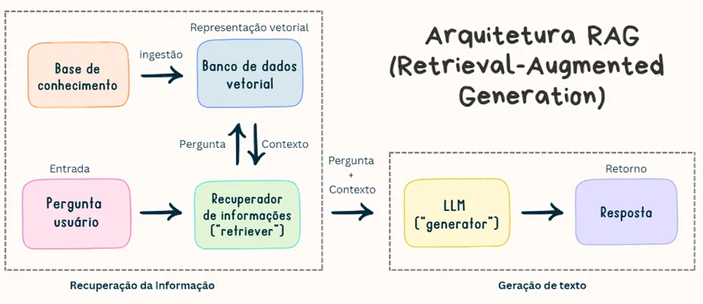
\includegraphics[width=125mm,keepaspectratio]{img/rag}
		\caption[Arquitetura \textit{RAG}]{Arquitetura \textit{RAG}}
		\label{fig:ragDiagram}
	\end{figure}
	
	Entre as principais vantagens desta arquitetura está a possibilidade de obter respostas mais relevantes e corretas, uma vez que o modelo passa a ter acesso a informação específica em vez de depender apenas do conhecimento que já possui. Outra vantagem é que a informação pode ser atualizada sem ser necessário voltar a treinar o modelo. No entanto, esta abordagem também tem algumas limitações. A qualidade da resposta depende da qualidade e da relevância dos documentos encontrados. Se forem recuperados documentos pouco relevantes ou se faltar informação importante, a resposta do modelo pode não ser útil. Além disso, um sistema de \gls{RAG} requer uma base de documentos bem organizada e implica ter em conta o tempo necessário para pesquisar a informação e os recursos utilizados \autocite{Reference1,Reference4}.
	
	%----------------------------------------------------------------------------------------
	\subsection{Estratégias de Recuperação em Sistemas \gls{RAG}}
	
		Tal como o próprio termo indica, o \textit{Retrieval-Augmented Generation} descreve uma abordagem em que o modelo procura primeiro informação relevante (\textit{Retrieval}), utiliza essa informação para complementar o contexto (\textit{Augmented}) e, por fim, gera uma resposta com base nesse contexto (\textit{Generation}). A forma como a informação é recuperada pode variar de acordo com os dados disponíveis e com o objetivo da aplicação, sendo possíveis diferentes estratégias:
		
		\begin{itemize}
			\item \textbf{Recuperação por informação estruturada:} utiliza apenas campos selecionados e dados filtrados para encontrar informação relevante.
			\item \textbf{Recuperação semântica:} utiliza \textit{embeddings} (representações de objetos) para encontrar informação com significado semelhante ao conteúdo que está a ser analisado, mesmo quando são utilizadas palavras diferentes.
			\item \textbf{Recuperação híbrida:} combina informação estruturada com pesquisa semântica, permitindo primeiro limitar os resultados com base em determinados campos e depois encontrar os conteúdos mais semelhantes.
		\end{itemize}
		

%----------------------------------------------------------------------------------------
\section{Fine-tuning}
	
	O \textit{fine-tuning} consiste em adaptar um modelo de linguagem pré-treinado a uma tarefa ou domínio específico através de um novo treino com dados direcionados. Este processo permite que o modelo aprenda padrões e termos próprios do domínio, tornando as suas respostas mais adequadas ao objetivo pretendido.
	
	Apesar das suas vantagens, o \textit{fine-tuning} requer dados de treino de qualidade e recursos computacionais. Além disso, quando a informação do domínio muda frequentemente, é necessário voltar a treinar o modelo para acompanhar essas alterações. Por isso, em contextos com informação dinâmica, como a gestão de incidentes, o \gls{RAG} pode ser uma abordagem mais adequada para fornecer informação atualizada, enquanto o \textit{fine-tuning} pode ser usado como complemento para melhorar a consistência das respostas \autocite{Reference7}.
